\chapter{Documentation}\label{ch:documentation}
\lstset{style=block}

This chapter documents the hardware and software of the Raspberry Pi Cybersecurity Lab (RCSL), wherein the hardware section describes the hardware components, which the device is built from, and the software section explains the architecture of the software and its functionality.

\section{Hardware}
The figure below shows the hardware components used in the project, which are a Raspberry Pi (RPI), a USB network card, an ESP32 microcontroller, a display and a rotary encoder.

\begin{figure}[h]
    \centering
    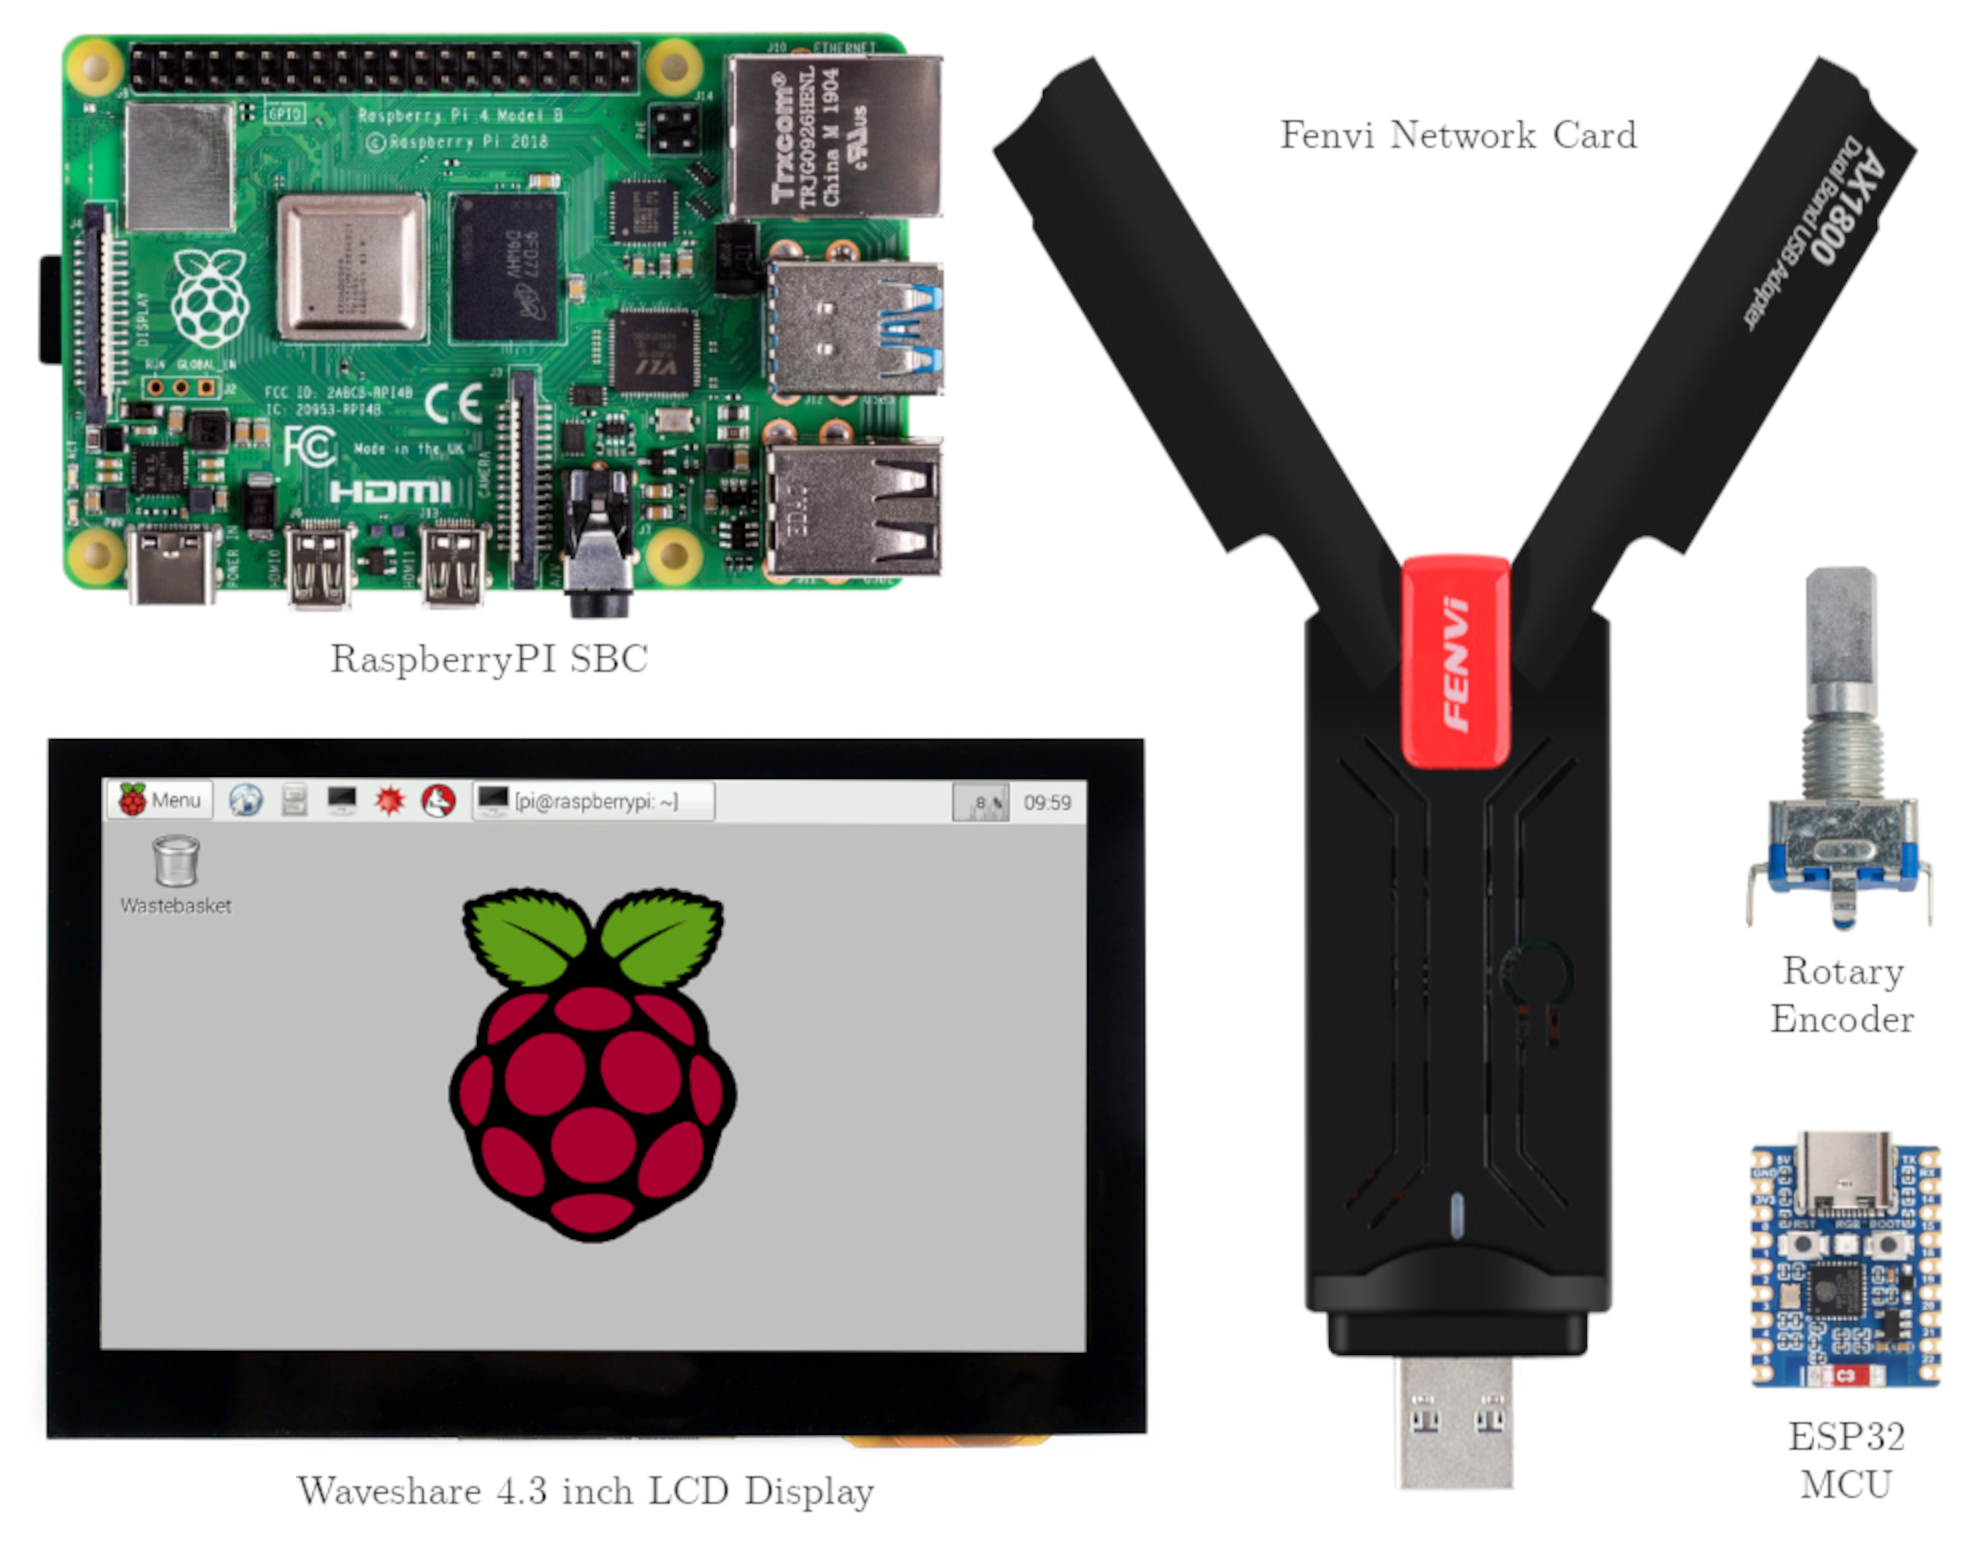
\includegraphics[width=0.8\linewidth]{figures/Abbildungen/Devices.png}
    \caption{Hardware Components}
    \label{fig:components}
\end{figure}

As the main computer, the Raspberry Pi 4B with 8GB of RAM was chosen due to its ease of use, Linux based operating system and widely available documentation. 

The RPI has an integrated Wi-Fi and Bluetooth card, as well as onboard Ethernet networking.
However, to support all Wi-Fi standards, an external network card is needed since the internal card of the RPI does not support the ciphers used by WPA3.
The Fenvi AX1800 USB Wi-Fi card was chosen for its compatibility with the Linux kernel, according to \cite{morrownr_USB_WiFi}, and low cost.

For some types of attack, such as cracking WPA/WPA2\footnote{see \cref{ch:testing}}, a Wi-Fi station, which is connected to the test network is needed, which in this case is an ESP32 microcontroller unit (MCU).
Selecting from the large offer of ESP32 MCUs, again size was taken into account and the ESP32-C6 Mini by Waveshare was chosen for its small size and good feature set.
It connects to the RPI's GPIO\footnote{General Purpose Input/Outputs can be configured to read or write data} pins using jumper cables (see \cref{fig:RCSL_nocase}), which supply the ESP32 with power and establish an UART\footnote{Universal Asyncronous Receiver/Transmitter is a bus standard for serial communication between embedded devices} connection.

Another device connected to the RPI's GPIO header is the rotary encoder.
On its five pins, it receives 3.3V supply voltage and outputs a gray code, indicating the direction of rotation, on two of its outputs. 
The fifth pin is used as the input for the push-button action of the encoder.

The hardware components are mounted in a 3D printed case, shown in \cref{fig:RCSL_side}.
\begin{figure}[h]
    \centering
    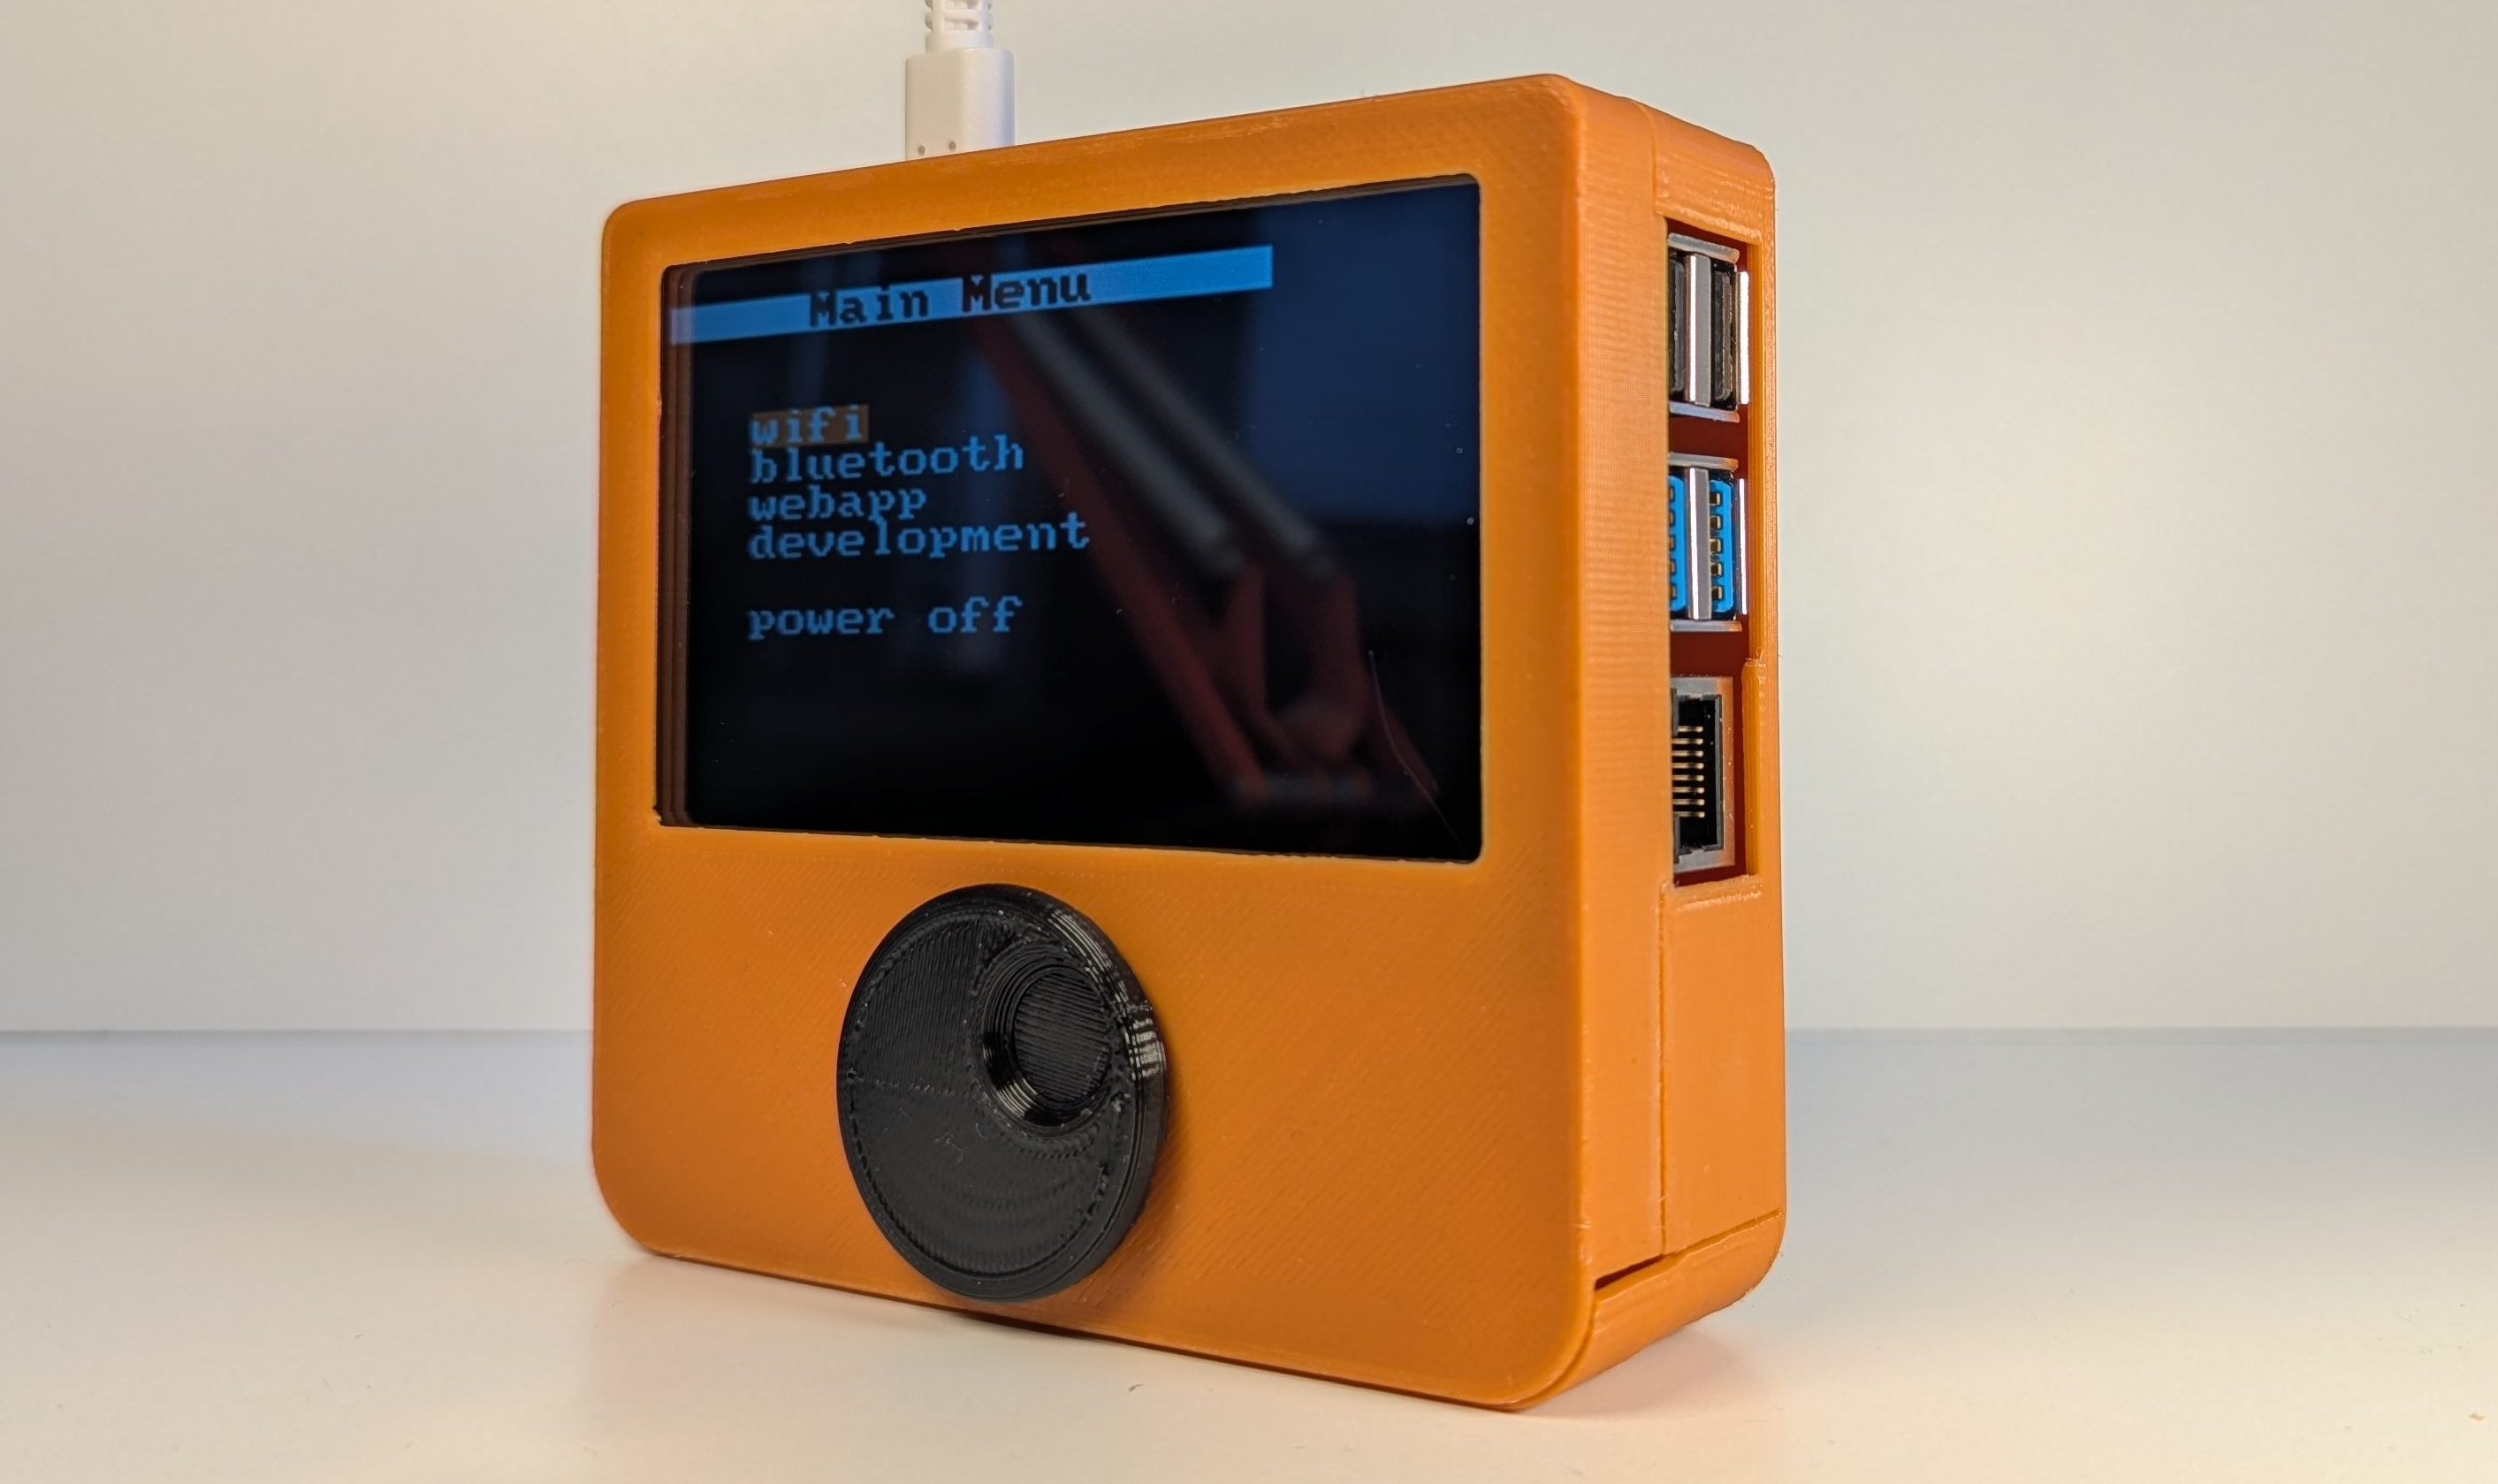
\includegraphics[width=0.90\linewidth]{figures/Abbildungen/Photo_Side.jpg}
    \caption{RCSL within its case}
    \label{fig:RCSL_side}
\end{figure}

\newpage
\section{Software}

\textit{Note: The project does not focus on performance or software quality.
It is written to implement the wanted functionality and should be seen as experimental, since it is neither optimised for performance nor have proper error handling mechanisms been implemented.}

\subsection{Overview}
The software of the project is mostly modular, and it consists of a central program, which runs the user interface (UI) and then executes various shell scripts\footnote{chain of commands to execute in the terminal of a Linux/Unix system}, with which the functionality is implemented.
As can be seen in \cref{fig:architecture}, besides the UI program, there are programs for MQTT communication and input processing, also the services of the Network Manager and the Juice Shop project are used. 

\begin{figure}[h]
    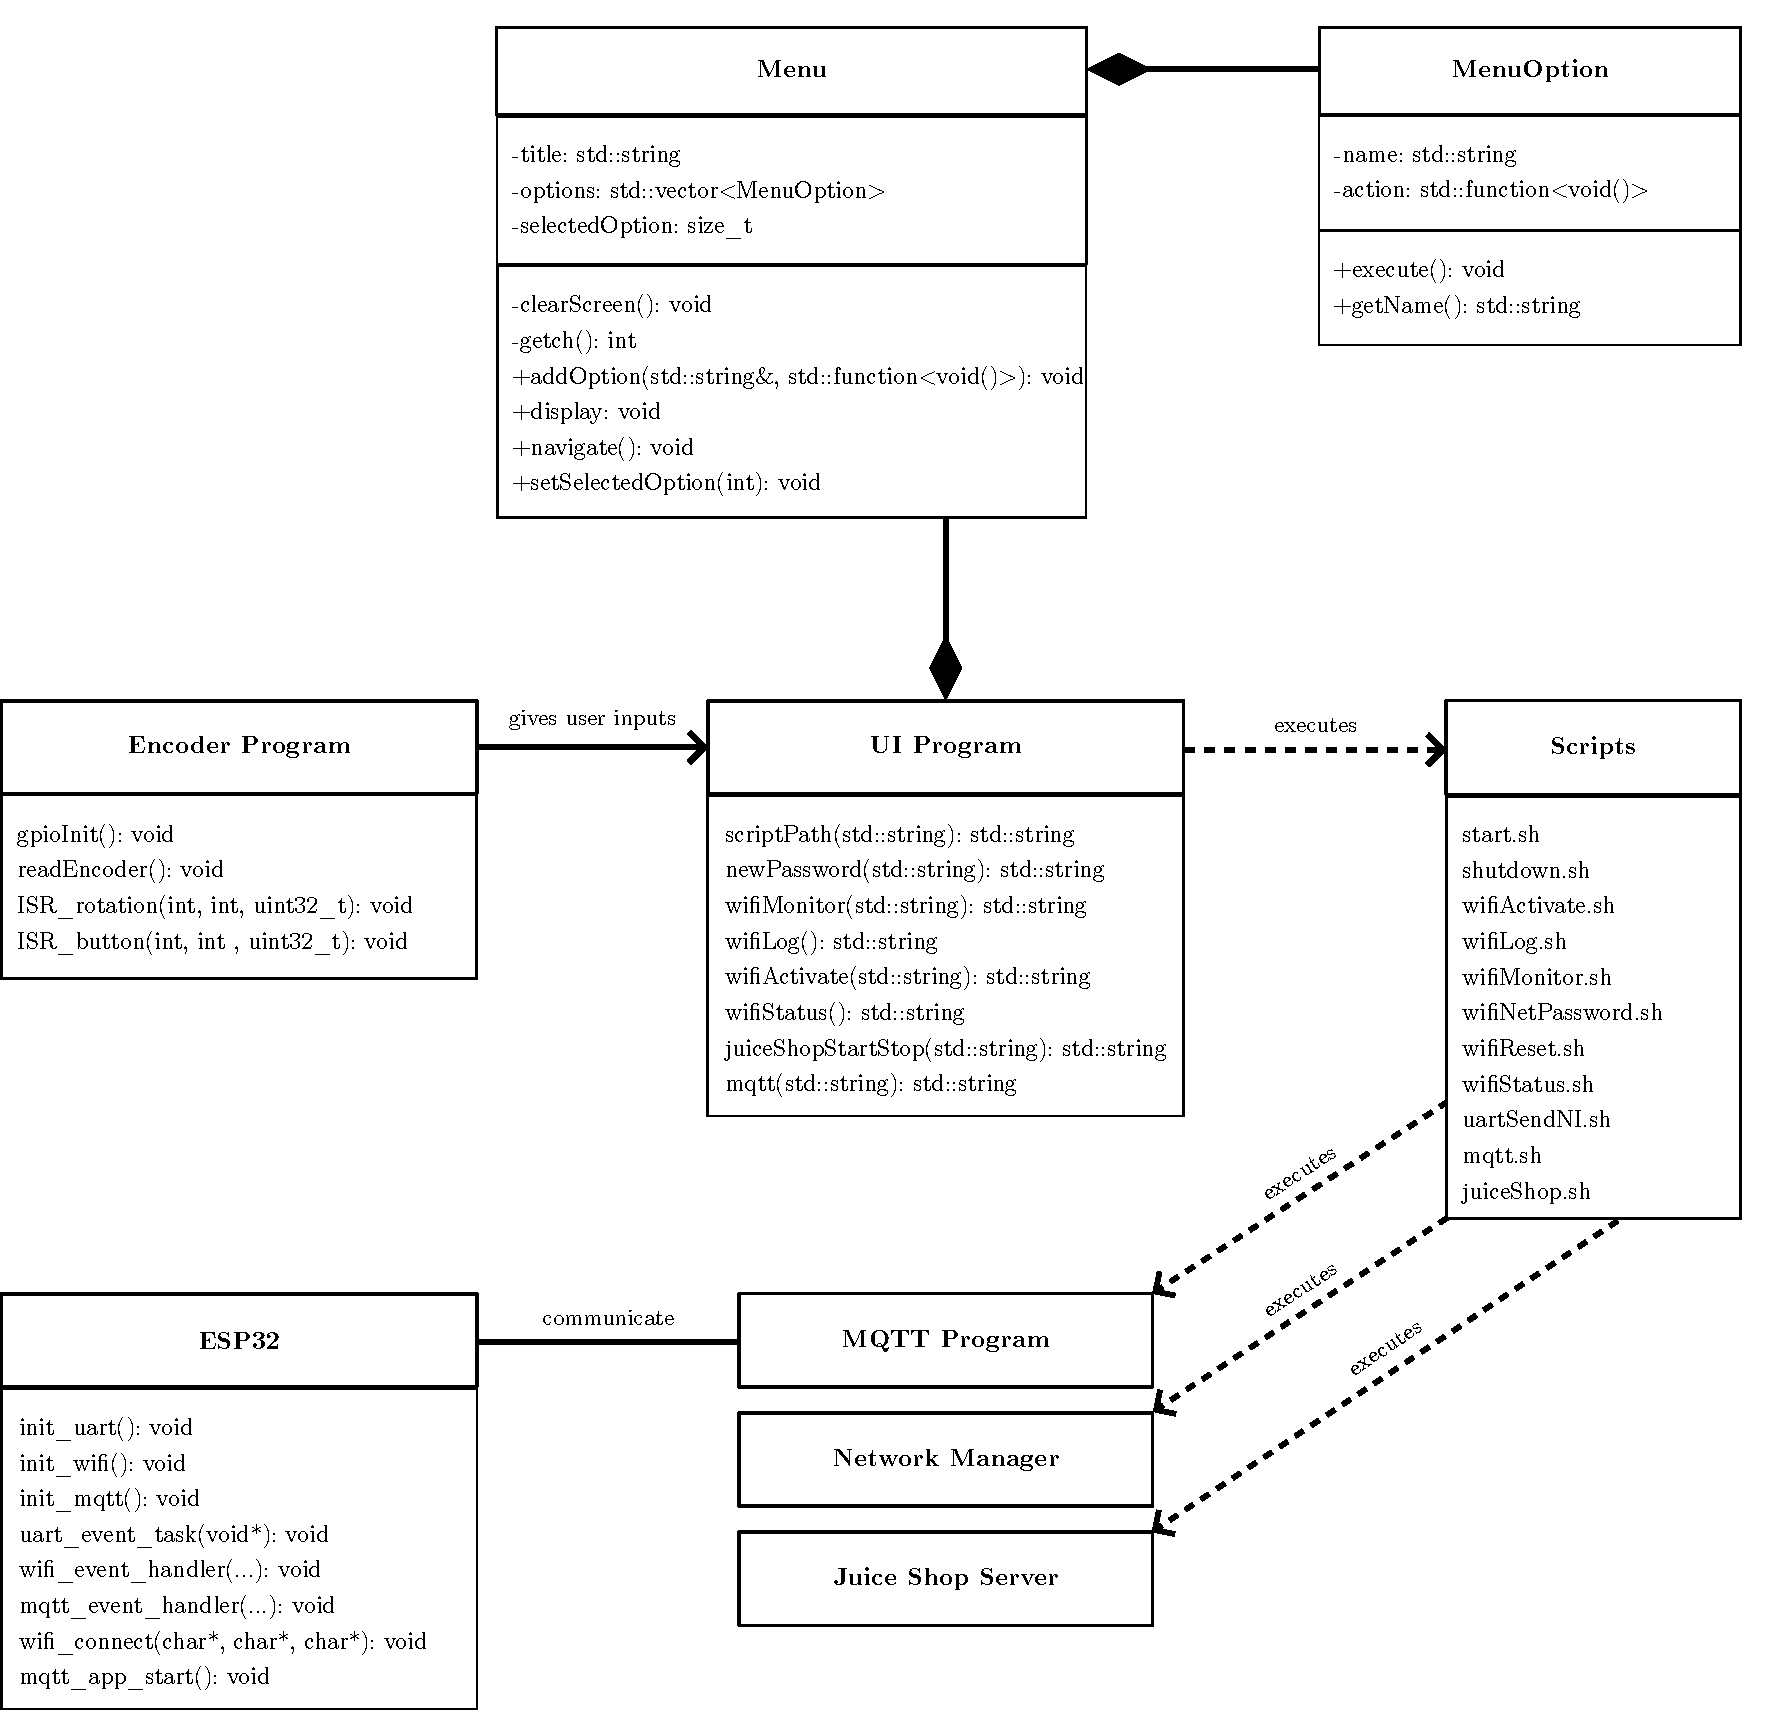
\includegraphics[width=\linewidth]{figures/Abbildungen/architecture.pdf}
    \centering
    \caption{Software Architecture}
    \label{fig:architecture}
\end{figure}

\textit{Note: Only the UI program is written object-oriented and only Menu and MenuOption are object classes.}


\subsection{UI Program}

Upon booting the device, a systemd service executes start.sh, which starts the encoder program and the UI program, with the output of the encoder program piped into the input of the UI.
The UI displays the main menu, depicted in \cref{fig:menu_main}, which the user can interact with by using the rotary encoder.
Each page of the UI is a "Menu" object, each menu has a title, options stored inside a vector of the type "MenuOption", a variable to track the currently selected option, a method to add options to a menu, and methods for navigation, input capture and displaying.
%The program starts by calling the display() function of the main menu, which then prints the options of the menu periodically, highlighting the selected option in orange.
MenuOption objects have a name, as well as an action of the std::function type, which can be executed by calling the execute() method.
In the main of the program, the constructors for menus and the addOption() methods are being used to create the different menus and their submenus.
An overview of the menus and options, currently present inside the UI program can be seen in \cref{ssec:A_docu_software}.
The program starts by calling the navigate() function of the main menu, which then displays all available submenus and menu options.
All submenus work in the same way as the main menu, getting their respective navigate() called upon selection.
During navigation, the UI periodically prints the available options, using Unicode to highlight the currently selected option as well as to give contrast to the title of the menu (see \cref{fig:menu_main}).

\begin{figure}[h]
    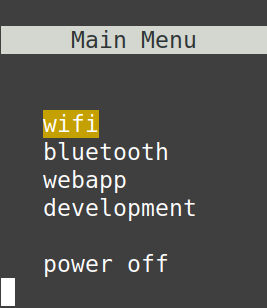
\includegraphics[width=0.3\linewidth]{figures/Abbildungen/hackerypi/menu_main.png}
    \centering
    \caption{Main Menu}
    \label{fig:menu_main}
\end{figure}

\textit{More examples for the UI can be found in the appendix, for example, \cref{fig:menus}.}

When an action, like activation of a network, is executed, main calls the according shell script with the system() function (see lis. \ref{lst:main_activateWEP}).
Scripts, which require an input, are called with a specific function that pipes the according information into the script (see lis. \ref{lst:main_wifiActivate}).

\lstinputlisting[language=C,linerange={29-32},caption={wifiActivate function in the UI program},label={lst:main_wifiActivate}]{listings/Raspi-CyberSec-Lab-Project/Program/main.cpp}

\lstinputlisting[language=C,linerange={98-98},caption={use of wifiActivate for WEP network},label={lst:main_activateWEP}]{listings/Raspi-CyberSec-Lab-Project/Program/main.cpp}

\subsection{Encoder Program}
For input, the RCSL uses a rotary encoder with a push-button, turning the encoder moves the menu selection up or down, the push-button executes the selected option (see \cref{fig:navigation}).
The encoder is connected to the Raspberry Pis GPIO interface, its rotation is segmented with clicks, similar to the scroll wheel of a computer mouse.
Like shown in \cref{fig:encoder_processing}, rotation between two clicks outputs one complete Gray code sequence on the signals DT and CLK, which is processed by the encoder program.
This happens within the rotation handling interrupt service routine (ISR), shown in lis. \ref{lst:ISR_rotation}, which is executed when DT outputs a high-low transition.

\begin{figure}[h]
    \centering
    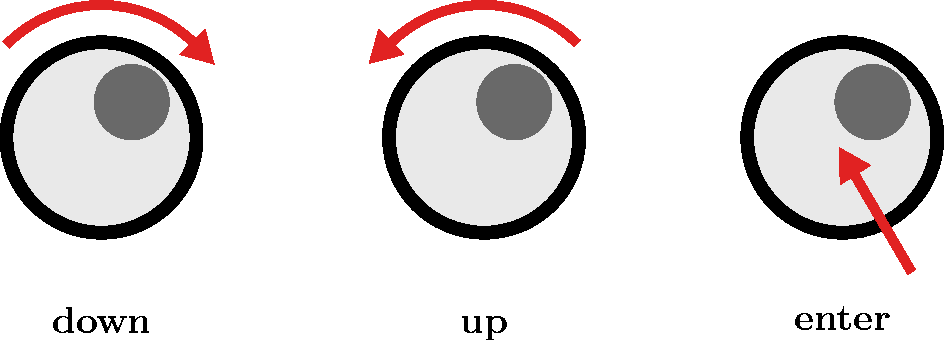
\includegraphics[width=0.5\linewidth]{figures/Abbildungen/navigation_engl.pdf}
    \caption{Navigation Scheme}
    \label{fig:navigation}
\end{figure}

The ISR checks the state of CLK, which determines the direction the encoder was turned: CLK=0 means the encoder has been turned clockwise, CLK=1 means counter-clockwise (see \cref{fig:encoder_processing}).
Subsequently, a command in the form of a string, representing an ANSI Escape Code, is printed.
Escape Codes are used as an output for peripheral buttons, which are not a character, for example, \lstinline[style=inline]|"\033[A"| describes the pressing of the downwards button on the keyboard.
As previously explained, the output of the encoder program is piped into the input of the UI, therefore rotating the encoder leads to the UI receiving the codes for up and down.
The push-button action is processed similarly, with an ISR outputting a newline symbol to the UI.

\newpage
\lstinputlisting[linerange={13-22},language=C,caption={Rotation handling ISR},label={lst:ISR_rotation}]{listings/Raspi-CyberSec-Lab-Project/Program/encoder.h}

Because the commands used for navigation are ordinary ANSI escape codes, the program can be easily tested on any computer by navigating the UI with the keyboard.

\subsection{Shell Scripts}

The wifiActivate.sh script is used to open Wi-Fi hotspots, where the user can choose the type of Wi-Fi standard being used. 
It receives an input command and then establishes a WEP, WPA, WPA2 or WPA3 network.
On first use, it sets up a network configuration, which just gets activated on repeated use, as seen for WEP networks in the code extract \ref{lst:wifiActivate.sh}.

\lstinputlisting[language=bash,linerange={1-18},caption={extract of wifiActivate.sh},label={lst:wifiActivate.sh}]{listings/Raspi-CyberSec-Lab-Project/Skripte/wifiActivate.sh}

After a Wi-Fi hotspot has been activated, a command with the connection details is sent to the ESP32 over UART.
This functionality is implemented by the uartSendNI.sh script, which gets called by wifiActivate.sh (see line 17 of lis. \ref{lst:wifiNewPassword.sh}).
Receiving the network information, the ESP32 will then connect to the provided network and act as a communication partner for the RPI.
    
With the wifiReset.sh script, the currently active network connection is turned off, which gets called by the deactivate option in the Wi-Fi menu.

To display the current status of the network, meaning its security standard, SSID and password, the wifiStatus.sh script is used.
It uses the \lstinline[style=inline]|nmcli dev wifi show-password| to output to the UI, which then looks like the following:

\begin{figure}[h]
    \centering
    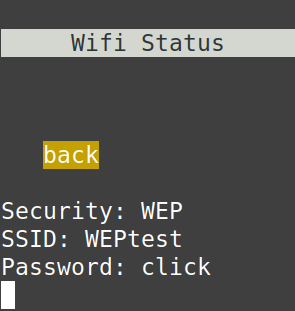
\includegraphics[width=0.24\linewidth]{figures/Abbildungen/hackerypi/status_wifi.png}
    \caption{Wi-Fi status menu}
    \label{fig:menu_status}
\end{figure}


When activating monitoring, wifiMonitor.sh uses the \lstinline[style=inline]|iw event -T| command to log devices connecting and disconnecting from the network.
Selecting the "monitor" option, the user is presented with the options of de-/activating the network monitoring as well as viewing or deleting the monitoring log.

Once a network has been cracked, the wifiNewPassword.sh script can be used to give a new random password to the selected network inside the change password menu.
The script then pulls a random password from a password list (see lis. \ref{lst:wifiNewPassword.sh}), containing popular passwords, that have been filtered to work with the specification of each network standard.
WEP networks use passwords with 5 or 13 characters, while WPA and WPA2 networks need passwords with at least 8 characters, and WPA3 networks work with passwords of every length.

\lstinputlisting[language=bash, linerange={8-10}, caption={extract from wifiNewPassword.sh}, label={lst:wifiNewPassword.sh}]{listings/Raspi-CyberSec-Lab-Project/Skripte/wifiNewPassword.sh}

\subsection{Bluetooth}
\textit{Note: the Bluetooth features, originally planned, have not been implemented due to time constraints and may be implemented in the future.}

\subsection{Juice Shop}\label{ssec:juice_shop}
Inside the webapp menu, the Juice Shop and MQTT communication can be found.

Juice Shop is a project by the Open Worldwide Application Security Project (OWASP).
It is "a web application with a vast number of intended security vulnerabilities, [which] is supposed to be the opposite of a best practice or template application for web developers: It is an awareness, training, demonstration and exercise tool for security risks in modern web applications" \cite{PWNING_JuiceShop}.
When activating the Juice Shop, the juiceShop.sh script will start up the server for the OWASP Juice Shop project and open a hotspot, which can be used to access the simulated webstore.

\textit{Note: further information about the project can be found in \cite{PWNING_JuiceShop}, which is the official companion to the Juice Shop.}

\subsection{MQTT Communication}
When a Wi-Fi network has already been activated from the Wi-Fi menu, a simulated MQTT communication can be started from the MQTT menu.
Starting a conversation will again send a command via UART to the ESP32, prompting it to connect to the MQTT broker, running on the RPI.
Following up, uart.sh starts the UART program, which begins an infinite MQTT conversation with the ESP32.

\subsection{ESP32}
The code for the ESP32 is based on the code examples provided by Espressif Systems on the official ESP-IDF GitHub \cite{espidf}.
It includes event handling for UART, Wi-Fi and MQTT and a client for MQTT.
The UART event handler has been modified to process the commands sent by the RPI and passes connection information to the Wi-Fi and MQTT instances.

\subsection{Miscellaneous}
The development menu contains options used during development, these can be adjusted on the fly inside the development.sh script.

When selecting the shutdown option, all running processes are stopped, and the shutdown.sh script calls \lstinline[style=inline]|shutdown now| to turn off the device.



